\documentclass[class=minimal,border=10pt]{standalone}
\usepackage{tikz}
\usepackage{xcolor}
% 数学符号(\mathbb, \mathcal 等)支持
\usepackage{amsmath,amssymb}
\definecolor{base03}{RGB}{0,43,54}
\definecolor{base02}{RGB}{7,54,66}
\definecolor{cyan}{RGB}{42,161,152}
\usetikzlibrary{calc,shapes,positioning,decorations.pathreplacing}
\begin{document}
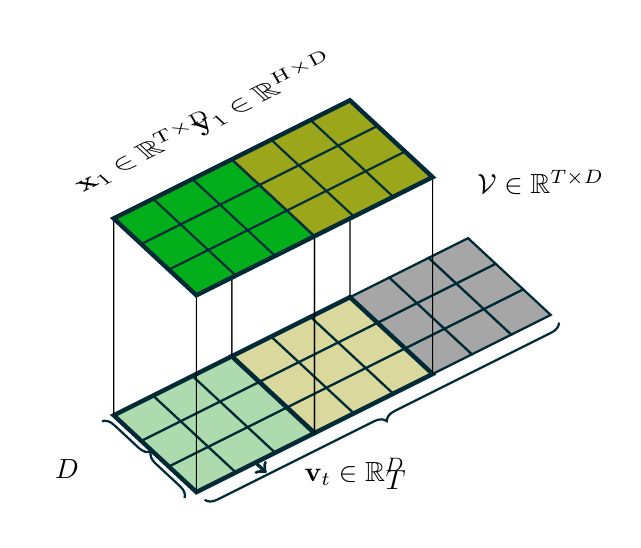
\begin{tikzpicture}[scale=.5, every node/.style={minimum size=1cm}, on grid]
    % 变量颜色定义(每个变量一种颜色,全局供输入/输出层使用)
    \definecolor{var0}{RGB}{38,139,210}
    \definecolor{var1}{RGB}{42,161,152}
    \definecolor{var2}{RGB}{133,153,0}
    % 立体:输入平面(1×1 方格,与卷积相同的斜视)
    \begin{scope}[node/.append style={yslant=0.5,xslant=-0.7},
                    yslant=0.5,xslant=-0.7]
        % 时间序列输入:每行一个变量,横轴为时间,1×1 方格
        \draw[draw=base03, fill=gray!70, thick] (0,0) rectangle (1,1);
    \draw[draw=base03, fill=gray!70, thick] (0,1) rectangle (1,2);
    \draw[draw=base03, fill=gray!70, thick] (0,2) rectangle (1,3);
    \draw[draw=base03, fill=gray!70, thick] (1,0) rectangle (2,1);
    \draw[draw=base03, fill=gray!70, thick] (1,1) rectangle (2,2);
    \draw[draw=base03, fill=gray!70, thick] (1,2) rectangle (2,3);
    \draw[draw=base03, fill=gray!70, thick] (2,0) rectangle (3,1);
    \draw[draw=base03, fill=gray!70, thick] (2,1) rectangle (3,2);
    \draw[draw=base03, fill=gray!70, thick] (2,2) rectangle (3,3);
    \draw[draw=base03, fill=gray!70, thick] (3,0) rectangle (4,1);
    \draw[draw=base03, fill=gray!70, thick] (3,1) rectangle (4,2);
    \draw[draw=base03, fill=gray!70, thick] (3,2) rectangle (4,3);
    \draw[draw=base03, fill=gray!70, thick] (4,0) rectangle (5,1);
    \draw[draw=base03, fill=gray!70, thick] (4,1) rectangle (5,2);
    \draw[draw=base03, fill=gray!70, thick] (4,2) rectangle (5,3);
    \draw[draw=base03, fill=gray!70, thick] (5,0) rectangle (6,1);
    \draw[draw=base03, fill=gray!70, thick] (5,1) rectangle (6,2);
    \draw[draw=base03, fill=gray!70, thick] (5,2) rectangle (6,3);
    \draw[draw=base03, fill=gray!70, thick] (6,0) rectangle (7,1);
    \draw[draw=base03, fill=gray!70, thick] (6,1) rectangle (7,2);
    \draw[draw=base03, fill=gray!70, thick] (6,2) rectangle (7,3);
    \draw[draw=base03, fill=gray!70, thick] (7,0) rectangle (8,1);
    \draw[draw=base03, fill=gray!70, thick] (7,1) rectangle (8,2);
    \draw[draw=base03, fill=gray!70, thick] (7,2) rectangle (8,3);
    \draw[draw=base03, fill=gray!70, thick] (8,0) rectangle (9,1);
    \draw[draw=base03, fill=gray!70, thick] (8,1) rectangle (9,2);
    \draw[draw=base03, fill=gray!70, thick] (8,2) rectangle (9,3);
        % 输入网格线(1×1)
        \draw[step=1, base03, thin] (0,0) grid (9, 3);
        % X 窗口高亮(绿色,对应 X_i)
        \draw[base03, ultra thick, fill=green!30, fill opacity=0.6] (0, 0) rectangle (3, 3);
        \draw[step=1, base03, thick] (0, 0) grid (3, 3);
        % 保存 X 窗口四角坐标,用于与输出层连线
        \coordinate (XWBL) at (0, 0);
        \coordinate (XWBR) at (3, 0);
        \coordinate (XWTL) at (0, 3);
        \coordinate (XWTR) at (3, 3);
        % Y 窗口高亮(黄色,对应 Y_i)
        \draw[base03, ultra thick, fill=yellow!40, fill opacity=0.6] (3, 0) rectangle (6, 3);
        \draw[step=1, base03, thick] (3, 0) grid (6, 3);
        % 保存 Y 窗口四角坐标,用于与输出层连线
        \coordinate (YWBL) at (3, 0);
        \coordinate (YWBR) at (6, 0);
        \coordinate (YWTL) at (3, 3);
        \coordinate (YWTR) at (6, 3);
        % 输入层尺寸与轴标注:长为 T,宽为 D,V \in R^(T×D),以及 v_t \in R^D
        % T 方向括号(沿时间轴,位于输入平面下方)
        \draw[decorate,decoration={brace,mirror,amplitude=4pt},base03,thick]
            (0,-0.3) -- (9,-0.3);
        \node[below=6pt] at (4.5, -0.8) {$ T $};
        % D 方向括号(沿特征维度,位于输入平面左侧)
        \draw[decorate,decoration={brace,mirror,amplitude=4pt},base03,thick]
            (-0.3,0) -- (-0.3,3);
        \node[left=6pt] at (-0.8, 1.5) {$ D $};
        % 这里直接使用预先构造好的数学标签文本,避免在模板中出现未转义花括号
        \node[above right=4pt] at (9, 3.3) {$ \mathcal{V} \in \mathbb{R}^{T \times D} $};
        % 选取某一时刻的向量 v_t(D 维)
        \draw[->, very thick, base03] (1.5, 0.0) -- (1.5, -0.4);
        \node[right=4pt] at (1.8, -0.6) {$ \mathbf{v}_t \in \mathbb{R}^{D} $};
    \end{scope}
    % 立体:输出层(长方形格子,变量数不变,上下同变量同色)
    \begin{scope}[xshift=0, yshift=5cm,
                    every node/.append style={yslant=0.5,xslant=-0.7},
                    yslant=0.5,xslant=-0.7]
        % 输入窗口到输出单元的连线(输出层用长方形,高 OUTPUT_HEIGHT)
        % X -> 输出 X 块 (绿色,宽 kernel_size)
        \draw (XWBL) -- (0, 0)
              (XWBR) -- (3, 0)
              (XWTL) -- (0, 3.0)
              (XWTR) -- (3, 3.0);
        % Y -> 输出 Y 块 (黄色,宽 kernel_size)
        \draw (YWBL) -- (3, 0)
              (YWBR) -- (6, 0)
              (YWTL) -- (3, 3.0)
              (YWTR) -- (6, 3.0);
        % 输出:两个与输入窗口同尺寸的块,X 在前/左,Y 在后/右
        \draw[draw=base03, fill=green, thick] (0,0) rectangle (3,3.0);
        \draw[draw=base03, fill=yellow, thick] (3,0) rectangle (6,3.0);
        \draw[xstep=1, ystep=1, base03, thick] (0,0) grid (6, 3.0);
        \draw[base03, fill=base02, fill opacity=0.4] (0, 0) rectangle (6, 3.0);
        \draw[base03, ultra thick] (0, 0) rectangle (6, 3.0);
        % 标签:每一帧标注 X_i 和 Y_i
        \node[above=4pt] at (1.5, 3.0) {$ \mathbf{x}_{1} \in \mathbb{R}^{T\times D} $};
        \node[above=4pt] at (4.5, 3.0) {$ \mathbf{y}_{1} \in \mathbb{R}^{H\times D} $};
    \end{scope}
\end{tikzpicture}
\end{document}
